% THIS IS SIGPROC-SP.TEX - VERSION 3.1
% WORKS WITH V3.2SP OF ACM_PROC_ARTICLE-SP.CLS
% APRIL 2009
%
% It is an example file showing how to use the 'acm_proc_article-sp.cls' V3.2SP
% LaTeX2e document class file for Conference Proceedings submissions.
% ----------------------------------------------------------------------------------------------------------------
% This .tex file (and associated .cls V3.2SP) *DOES NOT* produce:
%       1) The Permission Statement
%       2) The Conference (location) Info information
%       3) The Copyright Line with ACM data
%       4) Page numbering
% ---------------------------------------------------------------------------------------------------------------
% It is an example which *does* use the .bib file (from which the .bbl file
% is produced).
% REMEMBER HOWEVER: After having produced the .bbl file,
% and prior to final submission,
% you need to 'insert'  your .bbl file into your source .tex file so as to provide
% ONE 'self-contained' source file.
%
% Questions regarding SIGS should be sent to
% Adrienne Griscti ---> griscti@acm.org
%
% Questions/suggestions regarding the guidelines, .tex and .cls files, etc. to
% Gerald Murray ---> murray@hq.acm.org
%
% For tracking purposes - this is V3.1SP - APRIL 2009

\documentclass{acm_proc_article-sp}

\begin{document}

% set the path for graphics
\graphicspath{{figures/}}

\title{User-Device Physical Unclonable Functions (UD-PUFs) based on Mobile Device Touchscreen Pressure}
%\subtitle{[Extended Abstract]
%\titlenote{A full version of this paper is available as
%\textit{Author's Guide to Preparing ACM SIG Proceedings Using
%\LaTeX$2_\epsilon$\ and BibTeX} at
%\texttt{www.acm.org/eaddress.htm}}}
%
% You need the command \numberofauthors to handle the 'placement
% and alignment' of the authors beneath the title.
%
% For aesthetic reasons, we recommend 'three authors at a time'
% i.e. three 'name/affiliation blocks' be placed beneath the title.
%
% NOTE: You are NOT restricted in how many 'rows' of
% "name/affiliations" may appear. We just ask that you restrict
% the number of 'columns' to three.
%
% Because of the available 'opening page real-estate'
% we ask you to refrain from putting more than six authors
% (two rows with three columns) beneath the article title.
% More than six makes the first-page appear very cluttered indeed.
%
% Use the \alignauthor commands to handle the names
% and affiliations for an 'aesthetic maximum' of six authors.
% Add names, affiliations, addresses for
% the seventh etc. author(s) as the argument for the
% \additionalauthors command.
% These 'additional authors' will be output/set for you
% without further effort on your part as the last section in
% the body of your article BEFORE References or any Appendices.

\numberofauthors{3} %  in this sample file, there are a *total*
% of EIGHT authors. SIX appear on the 'first-page' (for formatting
% reasons) and the remaining two appear in the \additionalauthors section.
%
\author{
% 1st. author
\alignauthor Timothy M. Dee\\
       \affaddr{Electrical \& Computer Engineering}\\
       \affaddr{Iowa State University}\\
       \affaddr{Ames, IA, USA}\\
       \email{deetimothy33@gmail.com}
% 2nd. author
%\alignauthor Ian T. Richardson\\
%       \affaddr{Electrical \& Computer Engineering}\\
%       \affaddr{Iowa State University}\\
%       \affaddr{Ames, IA, USA}\\
%       \email{ian.t.rich@gmail.com}
% 3nd. author
\alignauthor Akhilesh Tyagi\\
      \affaddr{Electrical \& Computer Engineering}\\
      \affaddr{Iowa State University}\\
       \affaddr{Ames, IA, USA}\\
       \email{tyagi@iastate.edu}
}

%\date{30 July 1999}
% Just remember to make sure that the TOTAL number of authors
% is the number that will appear on the first page PLUS the
% number that will appear in the \additionalauthors section.

\maketitle
\begin{abstract}
%TODO remove the last sentence, mabe?
Described in this document is a physical unclonable function (PUF) utilizing the variability derived from the pressure with which users interact with their mobile device touchscreens. We illustrate how a sequence of these pressure values from descrete touchscreen interactions may be used to uniquely characterize a user-device pair. This characterization method may find many applications in protecting access to a mobile device from a malicious party. As a result, the effectiveness of this scheme is described in terms of how one user may be differentiated from another.
\end{abstract}

% A category with the (minimum) three required fields
%\category{H.4}{Information Systems Applications}{Miscellaneous}
%A category including the fourth, optional field follows...
%\category{D.2.8}{Software Engineering}{Metrics}[complexity measures, performance measures]

%\terms{Theory}

%\keywords{physical unclonable function (PUF), mobile device authentication} % NOT required for Proceedings

\section{Introduction}
\label{sec:intro}
Mobile devices are ubiquitus in the modern world. These devices are becoming progressively more important for many applications with security sensative data. 
Securing mobile devices poses unique challenges and opportunities compared to traditional data security where it is difficult for an attacker to access the physical device on which the data is stored or from which the sensitive data may be accessed.
%

%TODO develop an understanding of the need for this system
The reality that an attacker may be able to gain access to a physical device makes securing any data stored on or accessed by a mobile device significantly more challenging. Traditional physical unclonable functions (PUFs) which can be used to uniquely to a given hardware device are no longer sufficient to guarentee the authenticity of a user.
%
This modivates an extension of the traditional PUF known as a user-device physical unclonable function(UD-PUF). This UD-PUF entangles the physical characteristics of the user in combination with the device to enable a more secure authentication scheme.

%TODO problem statement, describe what the UD-PUF must accomplish 


\section{Related Work}
\label{sec:related_work}
%TODO
%detail what was done in the sensec paper
%provide a brief history of UD-PUFS


%describe what touchscreen pressure is
%describe the physical component of the pressure (current at the edge of screen on android device)
\section{Touchscreen Pressure}
\label{sec:touchscreen}
%TODO 
%describe what is touchscreen pressure
If our goal is be be able to distinguish a user's interaction with a given device from this same user on a different devie and from different users on any device than our description of the user will need to be a product of both the user and the device. In the android operating system there exists a pressure function which returns a value proportional to current at sides of phone for a given touch screen interaction. \cite{zhu2013sensec} We will henseforth refer to this as touch pressure. 

%describe why touchscreen pressure is a good candidate for our UD-PUF
The pressure function is significant, because it's value not only depends on the characteristics of the device but also on the way in which a user interacts with a given device. The effect of a given device on the touch pressure value will differ significantly due to variations implicit in the manufacturing process for the touchscreens of these devices. \cite{manufacturing_differences} Our supposition is a given user will interact with a touchscreen in such a way as to cause significant variations in the touch pressure values when compared to other users \cite{user_touchscreen_interations}.  Given this, we have chosen touch pressure as the basis for our UD-PUF.

%describe a marcov model in general
%describe what it means to be an n-gram sliding marcov model
%describe in what way we a marcov model to describe a user, device pair (our marcov model of touch, pressure values.
%An n-gram sliding marcov model.
\section{Modeling a User-Device Pair}
\label{sec:modeling}
%describe the motivation for the use of a marcov chain
Interactions between useres and devices are complex. To interpret these actions in a meaningful way, in order to preform an authentication for example, it is necessary to simplify these interations. The chosen model must provide sufficient entropy such that a model generated with a given user-device pair is not consistantly reproducable by another user or on a different device. The modeling method must also be easily reproducable by the origional user on the origional device. A model having the neccessary characteristics required for this application is a Marcov Chain.

%TODO describe what is a marcov chain
Marcov Chains are useful in predicting systems who's behavior can be modeled in descrete states. The transitions between states can be identified to happen with some probability.

%Other information about marcov chains
%TODO traditional use of marcov chains
Historically the Marcov Chain has found applications in
%
Upon identification of an appropriate model the next step is to discover an optimal way in which it may be applied to the current problem. An interaction between a user and device can be described as a sequence of touch pressure values. Using a Marcov Chain to describe this sequence is only reasonable if we suppose that a given touch pressure value depends on some number of preceeding touch pressure values. \cite{marcov_chains_previous_n_values}
%

%n-gram a continuious sequence of n items
%markov model for comparason is built from a sliding model of the previous n touches
%describe how the marcov chain is applied to touch pressure to model a user
%this is a description of our specific implementation of a marcov model
\section{Touch Pressure Modeling}
%TODO
%describe the marcov model used
%
The goal in modeling a system with a marcov model is to classify the system in terms of its transitions between states. If such a model is to be used to purposes of uniquely identifying a given system, than the states of the model must be chosen in a way which exposes the uniqueness of the system.
The states of our marcov model are defined by the range in which

\section{Data Collection}
\label{sec:differentiation}
%TODO
%describe the number of users from which the data was collected
%describe the method of collection
%put the data in context by detailing the number of touches collected from each user and the number of touches used to build the model

%basically the authentication scheme used
%frame it in more general terms, independtant of our specific application
\section{Differentiating User-Device Pairs}
\label{sec:differentiation}

%this figure describes how false positive and false negative percentages vary based on authentication threshold
\begin{figure}
\centering
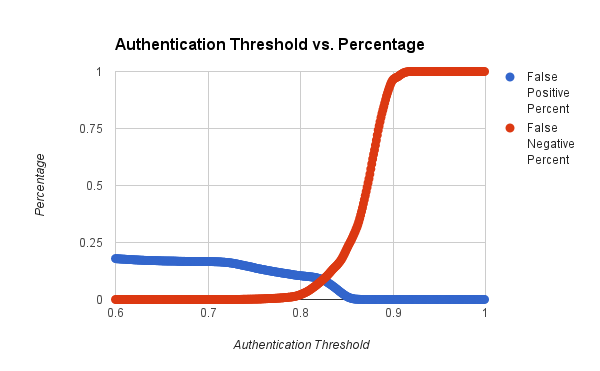
\includegraphics[width=3.9in]{threshold_vs_percentages.png}
\caption{Describes how false positive and false negative percentages vary as the authentication threshold is adjusted.}
\label{fig:threshold_vs_percentages}
\end{figure}

%TODO
%describe what the authentication threshold is
%define false positive
%define false negative
%explain why the intersection of these two is significant in choosing the authentication threshold
In distinguishing a particular user from another different user, it is necessary to develop a method of compairason between users. In our method of compairason we take the probability associated with a touch pressure coming after a sequence of preceding touch pressures for a particular user and compute the difference between this probability and the probability of the same touch pressure coming after the same sequence of touches for a different user. The average of these probability differences is taken to be the difference between two users.
%
Once a compairason is established a natural extension is a system of authentication. This system needs to determine when two sets of touch pressue values came from the same user-device pair. When authenticating a user, we take one minus the average difference between the model constructed from the two sets of touch pressure values. Take this value to be the authentication percentage for a given set of touch pressure values against another.
%
%TODO TODO add more metrics, and explain them, provide more graphs about them
To determine how well this system does at differentiating users it is useful to develop metrics which describe the system's performance under conditions which are similar to it's protential real-world applications. Figure \ref{fig:threshold_vs_percentages} illustrates how false positive percentage and false negative percentage vary based on where the threshold for authentication is set. 

%authentication threshold described
Here, authentication threshold refers to the value of authentication percentage one model must have against another for the models to be considered the same; two models which are the same are supposed to have been created from touches generated by the same user-device pair.
%false positive percentage described
False positive percentage measures what fraction of authentcations between two sets of touch pressures which did not come from the same user-device pair, therefore these sets should not be considered the same, but did authenticate as being the same in our authentication system.
%false negative percentage described
False negative percentage is exactly the inverse of false positive percentage in that it describes what fraction of authentications between two sets of touch pressures which did come from the same user-device pair, but did not authenticate as being the same in our authentication system.

%significance of the intersection of false positive, false negative values
In Figure \ref{fig:threshold_vs_percentages} there exists a clear intersection between false negative and false positive percentages. This intersection is significant; at this point the system nither biased toward allowing user-device pairs which should not authenticate to pass authentication nor toward disallowing user-device pairs, which should authenticate, from passing authentication. This point represents a balance allowing for %TODO

%what number of states exposed the most uniqueness e.g. how many tokens were best
%with what accuracy could users be destinguished from one-another
\section{Results}
\label{sec:results}


\section{Conclusions}
\label{sec:conclusions}


%possible, describe applications  in terms of continuious authentication
\section{Future Work}
\label{sec:futurework}

\bibliographystyle{abbrv}
\bibliography{bibliography/marcov_chains,bibliography/pufs,bibliography/other}
\end{document}
